\documentclass[11pt, class=article, crop=false]{standalone}
\usepackage{amsmath,amssymb,amsfonts,amsthm}
\usepackage{enumitem}
\usepackage{fancyhdr}
\usepackage{tikz-cd}
\usepackage{mathabx}
\usepackage{geometry}
\usepackage{color}
\usepackage{natbib}
\usepackage{braket}
\usepackage{graphicx}
\usepackage{hyperref}
\usepackage{cancel}
\usepackage{listings}
\usepackage{kiritsis}
\geometry{margin = 0.5in}

\begin{document}	

	\section*{Chapter 3: Quantization of Bosonic Strings} % (fold)
	\label{sec:chapter_3_quantization_of_bosonic_strings}
	
	\begin{enumerate}
		\item 
		For simplicity we will ignore the $\mu$ index in our calculation first.
		
   		First consider $[L_m, L_n]$ with $m+n \neq 0$. Then expanding in terms of commutators: This is the same as before, but now we must be careful about commutation: 
   	 \[
   	 		[L_m, L_n ] = \frac14 \sum_{k, l} [:\alpha_{m-k} \alpha_k: , :\alpha_{n-l} \alpha_l: ] 
   	 \]
   	 Note that the indices $m-k, k, n-l, l$ sum to $n+m$, if any pairwise sum of them is equal to zero (necessary for a nonvanishing commutator), then the other two will have sum equal to $n+m$. Then as long as $m+n \neq 0$ $\alpha_p$, there will be no normal-ordering ambiguity and we will recover the standard commutation relations as before. 
	 
	 So the remaining case to consider is $n = -m$. Take $m$ positive WLOG. The logic of the question from last chapter applies, but now we must be careful about the ordering of the $\alpha_i$ outside of the commutator. 
	 \begin{equation}
	 	\begin{aligned}
	 		\, [L_m, L_{-m}] &= \frac14 \sum_{k, l} [\alpha_{m-k} \alpha_k, \alpha_{-m-l} \alpha_l]\\
			&= \frac14 \sum_k \alpha_{m-k} \alpha_l k \delta_{k-m-l} 
				+ \alpha_{-m-l} \alpha_k (m-k) \delta_{m-k+l} 
				+ \alpha_{-m-l} \alpha_{m-k} k \delta_{k+l}
				+ \alpha_k \alpha_l (m-k) \delta_{k+l}\\
			&= \frac14 \sum_k \alpha_{m-k} \alpha_{k-m} k
				+ \alpha_{-k} \alpha_k (m-k)
				+ \alpha_{-m+k} \alpha_{m-k} k
				+ \alpha_{k} \alpha_{-k} (m-k)
	 	\end{aligned}
	 \end{equation}
	 We can split this into $k \geq 1$ and $k \leq 1$. The $k = 0$ term is already in normal order. When $k \geq 1$, the first, third, and fourth terms of the sum are out of normal order. The first term has only $m$ terms out of normal order. Rearranging these gives the constant:
	 \begin{equation*}
	 	\frac14 \sum_{k=1}^m k (k-m) = \frac14 \frac{m (m^2 - 1)}{6}
	 \end{equation*}
	 The fourth term has all terms out of normal order and gives the formally infinite sum
	 \[
	 	\sum_{k=1}^\infty k(m-k)
	 \]
	 The last term has all but the first $m$ terms out of normal order, and so contributes the sum
	 \[
	 	\sum_{k=m+1}^\infty (-m + k) k = - \sum_{k=1}^\infty (m-k) k + \sum_{k=1}^m (k-m) k
	 \]
	 The first part of this exactly cancels with the third term's infinite contribution. The last part of this gives exactly the same contribution as the first term. 
	 
	 Now, for $k \leq -1$ only the first two terms contribute. The first term contributes $\sum_k (m-k) k$ while the second term contributes $\sum_k (-k) (m-k)$ which cancel. Thus the term left behind is exactly:
	 \begin{equation}
	 	2 \times \frac14 \frac{m(m^2 - 1)}{6} = \frac{m(m^2 - 1)}{12}
	 \end{equation}
	 Note however that in fact our oscillators carry with them a $\mu$ index which we have ignored. If we incorporate it, then each normal ordering of $\alpha_i^\mu \alpha^j_\nu$ will include a factor of $\eta^{\mu \nu}$ which would have to be summed over. This will add in a copy of $D$ to our final result for the normal ordering term.
	 
	 Finally, we see that the normal ordering constant $a$ must be equal to:
	 \begin{equation}
	 	\frac12 \sum_{k} \alpha_{-k}^i \alpha^i_k \to \sum_{k=0} \alpha_{-k}^i \alpha^i_{k} + \frac12 \sum_{k>0} [\alpha^i_{k}, \alpha^i_{-k}] = :L_0: + \frac{D-2}{2} \underbrace{\sum_k k}_{\zeta(-1)} = -\frac{D-2}{24}
	 \end{equation}

	 
	 \item 
	 I believe that the treatment of the prior derivation of the central term was sufficiently careful, as I did not need to use any zeta regularization to compute an infinite sum. I only used zeta regularization in calculating the normal-ordering constant
	 % We can write:
% 	 \[
% 	 \begin{aligned}
% 		L_m &= \frac12 \sum_{n} \alpha_{m-n} \alpha_n =  \sum_{n \geq 1} \alpha_{-n} \alpha_{m+n} + \frac12 \sum_{i=0}^m \alpha_{m-i} \alpha_i\\
% 		L_{-m} &= \frac12 \sum_{n} \alpha_{-m-n} \alpha_n =  \sum_{n \geq 1} \alpha_{-n-m} \alpha_{n} + \frac12 \sum_{i=0}^m \alpha_{-m+i} \alpha_{-i}
% 	 \end{aligned}
% 	 \]
% 	 We have split the $L_m$ into an infinite (normal-ordered) sum and a finite (non-normal-ordered) one. The infinite sum gives contribution to the $[L_m, L_{-m}]$ commutator:
% 	 \[
% 	 	 \sum_{k, l \geq 1} [\alpha_{-k} \alpha_{m+k}, \alpha_{-l-m} \alpha_l]
% 	 \]
% 	 The terms $l, m+k$ are positive while $-k, -l-m$ are negative. Thus we have only two nonzero commutators:
% 	 \[
% 	 	 \sum_{k, l \geq 1} ( \delta_{k-l} (m+k) \alpha_{-k} \alpha_l + \delta_{k-l} (-k) \alpha_{-l-m} \alpha_{m+k}) = m \sum_{k\geq1} \alpha_{-k} \alpha_{k} + \sum_{k\geq 1}^m k \alpha_{-k} \alpha_k
% 	 \]
% 	 Note everything has remained in normal order. This term almost looks like $2 m L_0$.
%
% 	 In the cross term commutator between finite and infinite sums $L_m$'s finite sum term only has terms $\alpha_k$ with $0 \leq k \leq m$ while $L_{-m}$s infinite sum has no terms $\alpha_{-k}$ for those $k$ and vice versa for $L_{-m}$'s finite sum and $L_m$'s sum. Thus, there are no cross-terms and we have only to consider now the finite sum commutator:
% 	 	\[
% 	 		\frac14 \sum_{i,j=0}^{m} [\alpha_i \alpha_{m-i}, \alpha_{-m+j} \alpha_{-j}] = \sum_{i,j=0}^{\lfloor (m-1)/2 \rfloor} [\alpha_i \alpha_{m-i}, \alpha_{-m+j} \alpha_{-j}] + (( \frac14 [\alpha_{m/2} \alpha_{m/2}, \alpha_{-m/2} \alpha_{-m/2}] ))
% 	 	\]
% 		The double parentheses indicates that in the event of $m$ even, we get that extra term. In the sum, $m-i$ is never equal to $i$ and similarly for $-m+j$ and $-j$, so the only nonzero contributions to this first term are:
% 		\[
% 			\sum_{i,j=1}^{\lfloor (m-1)/2 \rfloor}  (\alpha_{-m+j}  \alpha_{m-i}[ \alpha_i, \alpha_{-j}] + [ \alpha_{m-i}, \alpha_{-m+j}] \alpha_{i} \alpha_{-j})  = \sum_{i=1}^{\lfloor (m-1)/2 \rfloor} (i \alpha_{-m+i} \alpha_{m-i} + (m-i) \alpha_{i} \alpha_{-i})
% 		\]
% 		The first part of this is normal ordered and so will vanish in the vacuum expectation value. The second is not. Normal ordering it gives an extra factor $\sum_{i=1}^{\lfloor (m+1)/2 \rfloor} (m - i) i$ and this gives the required $\frac{1}{12} m (m^2-1)$. When $m$ is even, the extra term contributes:
% 		\[
% 			\frac14 (\underbrace{2  \alpha_{-m/2} \alpha_{m/2}  m/2}_{\text{normal ordered}} + 2 \alpha_{m/2} \alpha_{-m/2}  m/2 ) \to \frac18 m^2
% 		\]
%
%
%
% 	I believe the above was the ``careful treatment'' that was asked for.
% 
	 \item Given that the Witt algebra is already given as an associative algebra, the commutator directly satisfies the Jacobi identity, since $(a- (b-c)) + (b-(c-a)) + (c-(a-b)) = a+b+c = 0$. Adding a central term gives 
	 \begin{equation}
	 	[L_a, [L_b, L_c]] + [L_b, [L_c, L_a]] + [L_c, [L_a, L_b]] = \frac{1}{12} \delta_{a+b+c} (a(a^2-1) (b-c) + b(b^2-1) (c-a) - c(c^2-1) (a-b) )
	 \end{equation}
	 This is zero by algebra. 
	 
	 \item For the closed string, we have:
	 \[
	 \begin{aligned}
		\dot X^\mu(\tau, \sigma) &= \ell_s^2 p^\mu + \frac{\ell_s}{\sqrt 2} \sum_{n \neq 0} (\alpha_n^\mu e^{-in\sigma} + \bar \alpha_{n}^\mu e^{i n \sigma}) e^{- i n \tau}\\
		{X'}^\mu (\tau, \sigma) &= \frac{\ell_s}{\sqrt2} \sum_{n \neq 0} (\alpha_n^\mu e^{-in \sigma} - \bar \alpha_{n}^\mu e^{i n \sigma} ) e^{-in\tau}
	 \end{aligned}
	 \]
	 Taking $X^+ = x^+ + \ell_s p^+ \tau$ sets $\alpha_n^+, \bar \alpha_n^+ = 0$ for all $n \neq 0$.
	 \[
	 \begin{aligned}
	 	\dot X^\mu + {X'}^\mu &= \ell_s^2 p^\mu + \sqrt2 \ell_s \sum_{n \neq 0} \alpha_n^\mu e^{-in\sigma} e^{-in\tau}\\
		\dot X^\mu - {X'}^\mu &= \ell_s^2 p^\mu + \sqrt2 \ell_s \sum_{n \neq 0} \bar \alpha_n^\mu e^{in\sigma} e^{-in\tau}
	 \end{aligned}
	 \]
	 Let's just look at the constraint $(\dot X + X')^2 = 0$ and then the other constraint will give the same result for the right-movers. 
	 \[
	 	0 = \ell_s^4 p^2 + \sqrt2 \ell_s^3 \sum_{n \neq 0} p \cdot \alpha_n e^{-in (\sigma + \tau)} + 2 \ell_s^2 \sum_{n, m \neq 0} \alpha_n \cdot \alpha_m e^{-i(n+m) (\sigma+\tau)}
	 \]
	 The zero mode gives $p^2 = 0$. Noting that $\alpha_n \cdot \alpha_m = - \alpha^+_{n} \alpha^-_m - \alpha^+_{m} \alpha^-_n + \alpha^i_n \alpha^i_m = \alpha^i_n \alpha^i_m$, we look at the remaining terms of each mode individually, so:
	 \[
	 \begin{aligned}
	 	0 &=\ell_s p \cdot \alpha_{n} + \sqrt2 \sum_{m} \alpha_{m-n}^i \alpha_m^i = - \ell_s p^+ \alpha^- +  \underbrace{\cancel{\ell_s p^i \alpha^i}}_{\alpha^i\text{ is transverse}} + \sqrt2 \sum_{m} \alpha_{m-n} \alpha_n\\
		& \Rightarrow \alpha^- = \frac{\sqrt{2}}{\ell_s p^+} \underbrace{\sum_{m} \alpha_{m-n}^i \alpha_m^i}_{2 L_0} = \frac{\sqrt{2}}{\ell_s p^+} \left[: \sum_{m} \alpha_{m-n}^i \alpha_m^i : - 2 a \delta_{n}\right]
	 \end{aligned}
	 \]
	 
	 \item Firstly, we see that $L_0 - \bar L_0$ can only differ by an integer, otherwise there's no combination of $\alpha_{-n} \bar \alpha_{-m}$ acting on $\ket{p^\mu}$ that will give a physical state. Now lets say they differ by an integer $n$. Then $\alpha_{-n}^i \bar \alpha_{-1}^i$ will be the lowest-lying excitation at level $(n+1, 1)$. We see there are $24$ of these that transform under $\mathrm{SO}(24)$, so they must give us a massless particle. We note also that we have exactly $24$ excitations at levels $(n+k, k)$ for $1 \leq k < n$, as the only way to get them is applying $\alpha_{-n-k}^i \bar \alpha_{-1-k}^i$. On the other hand, each of these has mass-shell condition:
	 \[
	 	0 = (L_0 - a) \alpha_{-n-k} \bar \alpha_{-k} \ket{p^\mu} \Rightarrow \ell_s^2 m^2 = 4 (n + k - a)
	 \]
	 However if this is massless for some value of $k$, it will be massive for $k+1$, breaking Lorentz invariance. 
	 
	 Note that $L - \bar L_0$ generates translations along $\sigma$ so this shows that any state should be invariant under $\sigma \to \sigma + c$.
	 
	 \item Note that $\mathrm{SO}(25)$ acts on $25 \times 25$ traceless symmetric tensors. Note that if we restrict to a subgroup $\mathrm{SO}(24)$ that leaves one of the spatial direction fixed, the $\mathrm{SO}(25)$ representation breaks down into two $\mathrm{SO}(24)$ representations: the symmetric tensor representation (including trace) on the 24 transverse directions, and the vector representation in those directions as well. This is exactly what we have at level two. So, we see we can arrange these two $\mathrm{SO}(24)$ rep'ns into the traceless symmetric $SO(25)$ tensor rep. 
	 
	 \item The generators (for the closed string) are:
	 \[
	 	J^{\mu \nu} = T \int_0^{2\pi} d\sigma (X^\mu \dot X^\nu - X^\nu \dot X^\mu) = x^\mu p^\nu - x^\nu p^\mu - i \sum_{n=1}^\infty [\alpha_{-n}^\mu \alpha^\nu_n - \alpha^\nu_{-n} \alpha^\mu_n + \overline{(\dots)} ]
	 \]
	 Upon computing the commutator $[J^{\mu \nu}, J^{\rho \sigma}]$ the $x^{ \mu} p^{\nu} - x^\nu p^\mu$ will give no problems, and there will be no cross terms between the right and left moving modes. So it is enough to look at the left movers.
	 \textbf{I'm gonna pass on doing this computation...}
	 
	 \item For NN boundary conditions, $\alpha_k^\mu$ is associated to the wavefunction $\cos(k \sigma), \sigma \in [0, \pi]$. This has eigenvalue $1$ under flip if $k$ is even and $-1$ if $k$ is odd. Thus this $\alpha_k$ must transform identically: $\Omega \alpha^\mu_k \Omega^{-1} = (-1)^k \alpha_k$. For DD boundary conditions, we have $\sin(k \sigma)$, which has opposite eigenvalues, so instead we get $(-1)^{k+1}$
	 
	 \item This is a Lie algebra of dimension $n(n-1)/2$, which already looks promising. In the case of all $\theta_i$ equal, we can pick basis so that the $R_{ij}$ are all $1$. This is clearly $\frak{so}(n)$. Now, take a diagonal unitary matrix $\gamma$ (note $\gamma^T = \gamma$). It clear that $\tilde \lambda_{ij} := \gamma^{1/2} \lambda_{ij} \gamma^{-1/2}$ gives the right structure under transposition:
	 \[
	 	\tilde \lambda^T = \gamma^{-1/2} \lambda^T \gamma^{1/2} = - \gamma^{-1/2} \lambda \gamma^{1/2} = - \gamma \tilde \lambda \gamma
	 \]
	 But since $\tilde \lambda_{ij}$ is just a conjugation action on the $\lambda_{ij}$, we will still have that the Lie algebra structure is preserved, and maintain $\frak{so}(n)$.
	 
	 For the second part, again when all the $\theta_i = 0$, this is just the definition of the symplectic group and we have $\lambda = - \omega \lambda^T \omega^{-1} = \omega \lambda^T \omega$ for $\omega$ the canonical symplectic written in the $(x_1, p_1, x_2, p_2, \dots)$ basis. Now note that the new symplectic form $\gamma$ can be written as $\sigma^{1/2} \omega \sigma^{-1/2}$ with $\sigma = \mathrm{diag}(e^{i \theta_1}, e^{i\theta_1}, e^{i \theta_2}, e^{i\theta_2}, \dots)$. Then define $\tilde \lambda = \sigma^{-1/2} \lambda \sigma^{1/2}$ and note that
	 \[
	 	\tilde \lambda^T = \sigma^{1/2} \lambda^T \sigma^{-1/2} = - \sigma^{1/2} \omega \lambda \omega \sigma^{-1/2} = - \gamma \tilde \lambda \gamma 
	 \]
	 as required. Again, conjugation action will preserve the Lie algebra structure, so this will remain $\frak{sp}(2n)$.
	 
	  % and we'll have:
% 	 \[
% 	 	[\lambda_{ij}, \lambda_{kl}] = i (\delta_{ik} \lambda_{jl} + \delta_{jl} \lambda_{ik} - \delta_{il} \lambda_{jk} - \delta_{jk} \lambda_{il})
% 	 \]
% 	 Now taking $\tilde \lambda_{i<j} = e^{\frac i2 (\theta_i - \theta_j)} \lambda_{i<j}$ and $\tilde \lambda_{i>j} = e^{-\frac i2 (\theta_i - \theta_j)} \lambda_{i>j}$ gives:
% 	 \[
% 	 	[\tilde \lambda_{i<j}, \tilde \lambda_{k<l}] = i e^{\frac i2 (\theta_i - \theta_j)} e^{\frac i2 (\theta_k - \theta_l)} (\delta_{ik} \lambda_{jl} + \delta_{jl} \lambda_{ik} - \delta_{il} \lambda_{j>k} - \delta_{jk} \lambda_{i<l})
% 	 \]
% 	 We see right away that the last two terms will absorb the exponentials. Our remaining terms look like:
% 	 \[
% 	 	i   (\delta_{ik} \tilde \lambda_{jl} e^{i \theta_i} e^{-i \theta_{\min (j, l)}}
% 		 + \delta_{jl} \tilde \lambda_{ik} e^{i \theta_j} e^{-i \theta_{\min (i, k)}}  - \delta_{il} \tilde \lambda_{j>k} - \tilde \delta_{jk} \lambda_{i<l})
% 	 \]
% 	 If $j < l$ and $k < $
%
	 \item In the symmetric case, we have $\lambda^T = \lambda$, so these are symmetric matrices of $N$ indices. Naturally $\mathrm{SO}(N)$ acts on these, and we see that they can be written as $\mathrm{F} \otimes \mathrm{F}$ for $\mathrm{F}$ the fundamental representation. This can be decomposed as the trivial representation and the traceless symmetric representation.  
	 
	 In the anti-symmetric case with $N$ even, I know that the symplectic group acts on $\mathbb R^{N}$. I'll call this the fundamental rep, and then note that tensoring it with its dual again gives an antisymmetric $N \times N$ matrix on which $\mathrm{Sp}(N)$ can act. This can be decomposed into the singlet and the skew-traceless antisymmetric matrix. 
	 
	 \item Traceless means that any pair of indices contracted with $\eta^{\mu \nu}$ gives zero. Locally, we can pick the metric so that only $\eta_{+-} = \eta_{-+} = 1$ is nonzero. This means that $T_{i_1 \dots i_n} = 0$ if any one $i$ is set to $+$ with the other set to $-$. Thus we can have only $T_{+\dots+}$ and $T_{-\dots-}$ nonzero. 
	 \item The round metric is
	 \[
	 	ds^2 = \frac{4 dz d\bar z}{(1+z \bar z)^2}
	 \]
	 The Lie derivative is:
	 \begin{equation}
	 	\mathcal L_{X} g_{ab} = X^c \partial_c g_{ab} + g_{ac} \partial_b X^c + g_{cb} \partial_a X^c
	 \end{equation}
	 % Now take $X = X^1 \partial_x + X^2 \partial_y$
	 % \[
	 % \begin{aligned}
	 % 	\mathcal L_{X} g_{11} &= (X^1 \partial_1 + X^2 \partial_2) g_{11} + g_{11} (\partial_1 X^1 + \partial_1 X^2) \Rightarrow - \frac{4 (x X^1 + y X^2)}{(1+x^2 + y^2)} + 2 \partial_1 X^1  = \lambda(x, y)\\
	 % 		\mathcal L_{X} g_{22} &= (X^1 \partial_1 + X^2 \partial_2) g_{22} + g_{22} (\partial_1 X^1 + \partial_1 X^2) \Rightarrow - \frac{4 (x X^1 + y X^2)}{(1+x^2 + y^2)} + 2 \partial_2 X^2 = \lambda(x, y)\\
	 % 		\mathcal L_{X} g_{12} &= g_{11} \partial_2 X^1 + g_{22} \partial_1 X^2 \hspace{1.28in} \Rightarrow \quad \partial_2 X^1 + \partial_1 X^2 = 0
	 % \end{aligned}
	 % \]
	 % Subtracting the first two gives $\partial_1 X^1 = - \partial_2 X^2$ while the second one gives $\partial_2 X^1 = \partial_1 X^2$. These look a lot like the Cauchy-Riemann equations.
	 %
	 Working with $z, \bar z$ we get:
	 \begin{equation}
		 \begin{aligned}
		 	\mathcal L_{X} g_{zz} &= 2 g_{z \bar z} \partial_z X^{\bar z} = 0 \\
			\mathcal L_{X} g_{zz} &= 2 g_{z \bar z} \partial_z X^{\bar z} = 0\\
			\mathcal L_{X} g_{z \bar z} &= (X^z \partial_z + X^{\bar z} \partial_{\bar z} ) g_{z \bar z} = \lambda(z, \bar z) g_{z \bar z}
		 \end{aligned}
	 \end{equation}
	 The first two equation shows us that $X^z, X^{\bar z}$ must be holomorphic and anti-holomorphic respectively. We want the function $\lambda$ to be well-defined on the entire Riemann sphere and so the last equation gives us:
	 \begin{equation}
	 	-2 \frac{ (X^z \bar z + X^{\bar z} z)}{1 + z \bar z} = \lambda(z, \bar z)
	 \end{equation}
	 We see that $X^z, X^{\bar z}$ cannot have any poles. Further, they cannot grow faster than $z^2, \bar z^2$  respectively as $z \to \infty$ otherwise $\lambda$ will blow up at the north pole. So our solutions space is spanned by $\partial_z, z \partial_z, z^2 \partial_z$ and their conjugates. 
	 
	 Next, right away we can see that the only nonzero Christoffel symbols in the round metric are $\Gamma^z_{zz}$ and $\Gamma^{\bar z}_{\bar z \bar z}$. Second, because $T$ is traceless, by the previous problem we see it has only two components: $T_{zz}$ and $T_{\bar z \bar z}$. Now looking at $\nabla^\beta T_{\alpha \beta}$ we see that this gives two equations:
	 \begin{equation}
	 	\begin{aligned}
	 		g^{z \bar z} \nabla_{\bar z} T_{zz} &= \partial_{\bar z} T_{zz} \\
			g^{z \bar z} \nabla_{z} T_{\bar z \bar z} &= \partial_z T_{\bar z \bar z}
	 	\end{aligned}
	 \end{equation}
	 Note that there can be no Christoffel contribution. This simply asks for globally-defined holomorphic 2-forms. Let's look at $T_{zz}$. Around $z = 0$, it must be a polynomial to avoid poles. Transforming to $w = 1/z, dw = - dz/z^2 \Rightarrow \frac{dz}{dw} = -z^2 = -w^{-2} $ we get $T_{ww}(w) = (\frac{dz}{dw})^2 T_{zz}(w)$. Note that the right hand side will only have poles at least as bad as $w^{-2}$ so we cannot have any global section of this vector bundle. Thus, there are no Teichmuller parameters.
	 
	 \item We can think of the torus as $\mathbb C / \Lambda$. Note that scaling and rotation preserve the complex structure of the fundamental parallelogram so WLOG we can pick $\Lambda = \mathbb Z\text{-span} \{1, \tau\}$ with $\tau \in \mathbb H$. Thus we need vector fields on $\mathbb C$ that respect the translation-invariance under $\Lambda$. Any translation-invariant holomorphic function is zero, we can only have the constant vector fields $\partial_z, \partial_{\bar z}$. 
	 
	  \begin{center}
	  	\includegraphics[scale=0.1]{"Drawings/Torus Killing"}
	  \end{center}
	 
	 We now look for holomorphic and anti-holomorphic traceless tensors. Again, $T_{zz}$ and $T_{\bar z \bar z}$ be translation-invariant w.r.t the lattice, so again they must be constants. We get $dz \otimes dz$ and $d \bar z \otimes d\bar z$ as our two Teichmuller deformations. As real tensors these are:
	 \[
	 	\begin{pmatrix}
	 		1 & 0\\
			0 & -1
	 	\end{pmatrix} = dx \otimes dx - dy \otimes dy, \quad 
	 	\begin{pmatrix}
	 		0 & 1\\
			1 & 0
	 	\end{pmatrix} = 2 dx \otimes dy ,
	 \]
	 \item Not sure exactly how they want us to calculate this. Let's assume they are OK with Gauss-Bonnet. For the disk with the flat metric, we have right away that the curvature $R$ vanishes. The geodesic curvature at the boundary is a constant, and is easily seen to be $1$. Integrating this over the boundary of the disk gives $2\pi$ so that $\chi=1$. 
	 
	 Using the round metric, it is quick to see that the only contribution to $R_{\mu \nu} = R^z_{\, \mu z \nu} + R^{\bar z}_{\, \mu \bar z \nu}$ is for $R^z_{z z \bar z} = -\partial_{\bar z} \Gamma^z_{z z}$
	  and $R^{\bar z}_{\bar z \bar z z} = \partial_z \Gamma^{\bar z}_{\bar z \bar z}$ giving $R_{z \bar z} = \frac{2}{(1 + |z|^2)}$. Tracing this gives $R = 1$. Integrating this over half the sphere gives $2 \pi$. The geodesic curvature vanishes on the great circle by symmetry, and we get $\chi = 1$ again.
	  
	  \item Any such surface can be decomposed as a sphere with $2n$ holes connected to $n$ handles. Let's integrate the scalar curvature over each piece individually. First the curvature integrated on the sphere with $2n$ disks removed is equal to the curvature integrated on the Riemann sphere: $4\pi$ minus the curvature integrated on $2n$ disks. We have just done this in the previous problem, and we get $2\pi \times 2n$. Lastly, the curvature on the handles is just the same as the curvature on the sphere with two holes cut out, which we have just calculated is $4 \pi - 2 \times 2\pi = 0$. Thus the total curvature is just $2 \pi (2-2n)$, giving us $\chi = 2-2n$ as required. 
	  
	  \begin{center}
	  	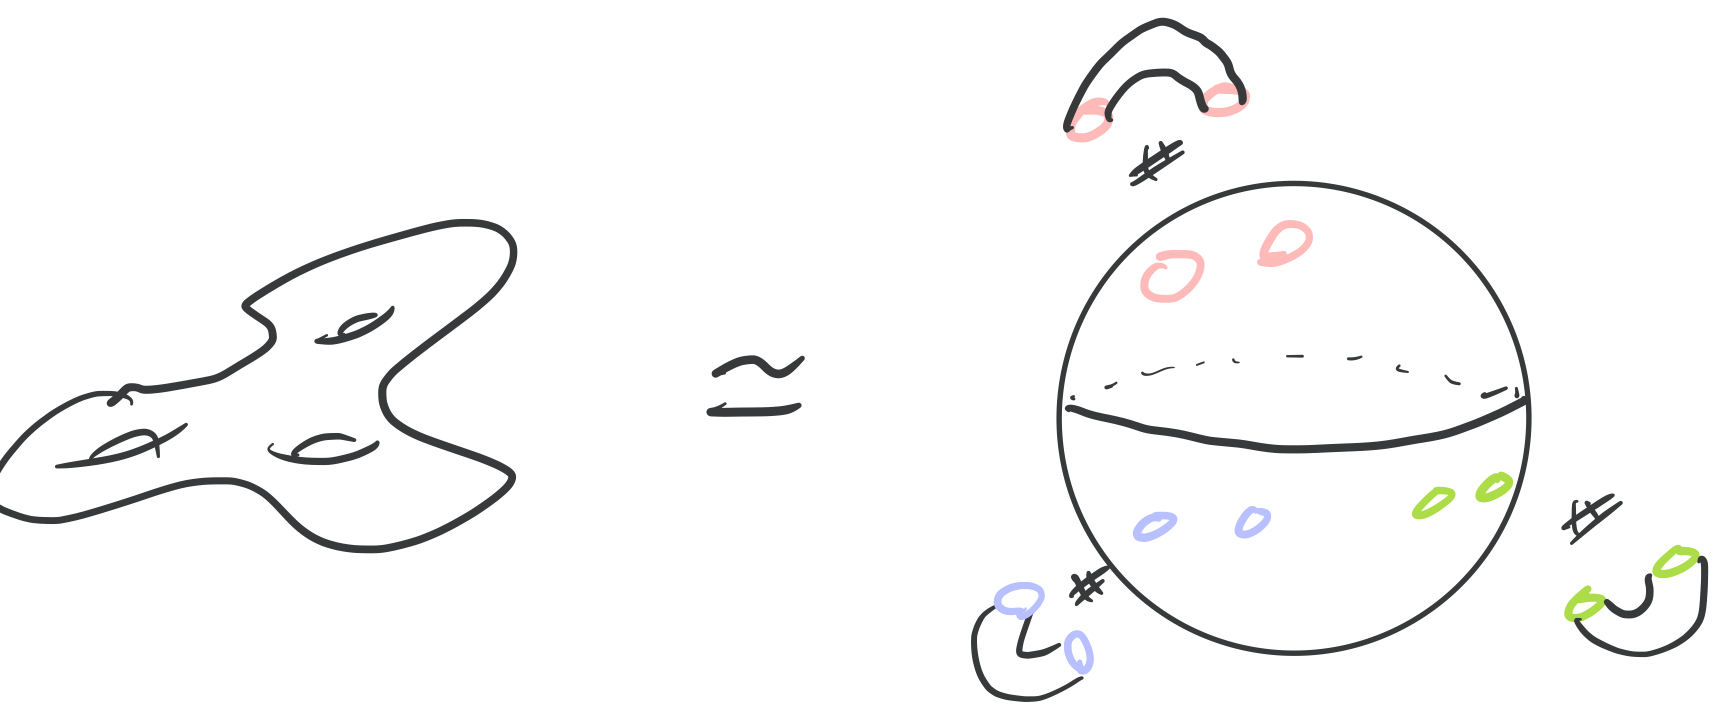
\includegraphics[scale=0.12]{Drawings/Handles}
	  \end{center}
	  
	  \item Our point particle action is $S_0 = \int d\tau e (e^{-2} (\partial_\tau x)^2 - m^2)$. Let's look at:
	  \[
	  	\int \frac{\mathcal D X \mathcal D e}{V_{gauge}} e^{-S_0} \sim \int \mathcal D X \mathcal D e \mathcal D b \mathcal D c \; e^{-S_0 - \int b (\delta F) c - i \int B F(e)}
	  \]
	  Note we don't need an $\alpha$ index on $B,b,c$ because they just parameterize the continuous symmetry with no discrete parameters:
	  \[
	  	(\delta_{\tau_1} \tau) (\tau) = \delta(\tau-\tau_1)
	  \]
	  Using Polchinski's convention for coordinate transformation (he also has $-B_A$ of Kiritsis), 
	  \[
	  	\delta_{\tau_1} X(\tau) = - \delta(\tau - \tau_1) \partial_\tau X , \qquad \delta_{\tau_1} e(\tau) = - \partial_\tau (\delta(\tau-\tau_1) e(\tau))
	  \]
	  and 
	  \[
	  	[\delta_{\tau_1} \delta_{\tau_2}](\tau) = - (\delta(\tau-\tau_1) \partial_\tau \delta (\tau - \tau_2) - \delta(\tau-\tau_2) \partial_\tau \delta(\tau-\tau_1) ) \, \partial_\tau \Rightarrow f_{\tau_1 \tau_2}^{\tau_3} = \delta(\tau_3-\tau_1) \partial_{\tau_3} \delta (\tau_3 - \tau_2) - \delta(\tau_3-\tau_2) \partial_{\tau_3} \delta(\tau_3-\tau_1)
	  \]
	  Then the BRST transformation is given by:
	  \begin{equation}\label{eq:polch}
	  	\begin{aligned}
	  		\delta_{\epsilon} X &= i \epsilon c \dot X\\
			\delta_{\epsilon} e &= i \epsilon \dot{(c X)}\\
			\delta_\epsilon   b &= \epsilon B_A\\
			\delta_\epsilon   c &= i \epsilon c \dot c\\
			\delta_{\epsilon} B &= 0
	  	\end{aligned}
	  \end{equation}
	  Now let's take $F(e) = e-1$. Then we get a ghost action
	  \[
	  \begin{aligned}
	  	b_A c^\alpha \delta_\alpha F^\alpha &\to \int d\tau_1 d\tau_2 b(\tau_1) c(\tau_2) \delta_{\tau_2}\, \left(1-e(\tau_2)\right) \\ &= \int d\tau_1 b(\tau_1) \partial_{\tau_1} \int d\tau_2 c(\tau_2) [\delta(\tau_1 - \tau_2) e(\tau_1)] = - \int d\tau \dot b c
	  \end{aligned}
	  \]
	  We enforce this constraint by integrating over $B$. Now we will have $\delta_\epsilon e = 0$ and $\delta_\epsilon b = i \epsilon (T^X + T^{gh})$. Because we are in Euclidean signature, we have $p = \partial_t X = i \dot X$ and similarly $p = -i c$ ($-i$ because the real time Lagrangian has term $-i \dot b c$). Then the BRST current (equal to charge because we're in 1D) is:
	  \[
	  	Q_B = p_X \delta_B X + p_b \delta_B b = - c \dot X^2 - i c i (- \frac12 \dot X + \frac12 m^2 - \dot b c) = - c \frac12 \dot X + \frac12 m^2 = c \frac12 (p^2 + m^2) = c H.
	  \]
	  Clearly $Q_B^2 = 0$.
	  As before, the ghosts generate a two-state system. Our set of states is given by $\ket{k^\mu, \uparrow}, \ket{k^\mu, \downarrow}$. Following convention, $c$ raises and $b$ lowers. $Q_B \ket{k, \downarrow} = \frac12 (k^2 + m^2) \ket{k, \uparrow}$ so all states of the form $\ket{k, \uparrow}$ with $k^2 + m^2 \neq 0$ are BRST exact. Similarly all states $\ket{k, \uparrow}$ are BRST closed along with all states of the form $\ket{k, \downarrow}$ with $k^2 + m^2 = 0$. So the closed states that are not exact are $\ket{k, \downarrow}$, $\ket{k, \uparrow}$ with $k^2 + m^2 = 0$. We take only the states with $b \ket{\psi} = 0$. The reason is that all states $\ket{k, \uparrow}$ are physical, and so we would need amplitudes between such states to be proportional to $\delta(k^2 + m^2)$ in order for the states to decouple, but \emph{amplitudes} cannot have such extreme singularities \textbf{Don't understand this. Appreciate it, and its relation to Siegel gauge.}.
	  
	  \item I believe these variations have Kiritsis taking $c \to -i c$ in his formalism. They also follow directly from Polchinski's formalism. Under a diffeomorphism $\delta_{\xi, \bar \xi} X = -\xi \d X - \bar \xi \bar \d X$. These are two copies of the reparameterization algebra developed in the previous problem, and so the commutation relations are the same. We get, again in Polchinski's formalism \eqref{eq:polch}
	  \begin{equation}
	  	\begin{aligned}
	  		\delta_{\epsilon} X &= i \epsilon (c \d X + \bar c \bar d X)\\
			\delta_\epsilon   c &= i \epsilon (c \partial c + \bar c \bar \partial \bar c)\\
			\delta_\epsilon   b &= i \epsilon (T^X + T^{gh})
	  	\end{aligned}
	  \end{equation}
	  
	  I see no problem with $Q^2_B$ giving zero when acting on the $X$ and $c$ fields.
	  \[
	  	\delta_B (c \d X+ \bar c \bar d X ) = i \epsilon (\cancel {c (\d c) \d X} + \cancel{\bar c (\bar \d \bar c) \bar \d X} - c \d (\cancel{c \d X} + \bar c \bar \d \bar c X) -  \bar c \d (\cancel{c \d X} + \bar c \bar \d \bar c X) )
	  \]
	  and the remaining terms die by the equations of motion. The $c$ variation will always die because we've already shown the transformations satisfy a Lie algebra with Bianchi identity. 
	  
	  It looks like the $b$ field will be nontrivial. If one of the equations of motion is the $T^X + T^{gh} = 0$ then this will be zero right away. Otherwise, we want to compute (WLOG in the holomorphic sector):
	  	  \[
	  	  	\delta_B (T^X + T^{gh}) = \delta_B (\frac1\alpha (\partial X)^2 + 2 b \partial c + \partial b c) = i \epsilon [\frac2\alpha \partial X \partial(c \partial X) + 2 (T^X + T^{gh}) \partial c + 2 b\, \partial(c \partial c) + \partial(T^X + T^{gh}) \partial c + \partial b\, c \partial c ] 
	  	  \]
		  The purely $b c$ terms cancel. I'm left with
		  \[
		  	\frac2\alpha [(\partial X)^2 \partial c + \partial X \partial^2 X c]
		  \]
		  I don't know how to get rid of this. I can write it as a total derivative less something proportional to $(\partial X)^2 \partial c$ and perhaps note that this is just $\partial c$ times the stress tensor, which perhaps vanishes classically? At any rate, there is no need to use $d=26$ here.
	  
	  \item Integrating over $\sigma$ will as usual pick out the zero mode. For $T_{++}$ this gives us
	  \[
	  	\sum_n (2 n b_{-n+m} c_n + n+m c_{-n} b_{n+m}) = \sum_n (m-n) :b_{n+m} c_{-n}:
	  \]
	  and similarly for the right-movers. To get the central charge we'll have to proceed as before, noting that only $[L_m, L_{-m}]$ can give a nonzero central term. As before, we expect only a finite part of the infinite sum to contribute to this. We thus take out the only terms of the sum with $m,n$ having the same sign:
	  \[
	  	\sum_{n=1}^m (m+n) b_{m-n} c_n , \qquad \sum_{n=1}^m (-2m+n) b_{-n} c_{-m+n}
	  \]
	  Then our commutators of these finite terms give:
	  \[
	  \begin{aligned}
	  		  	\sum_{k, k'} (m+k) (-2m + k') [b_{m-k} c_k, b_{-k'} c_{-m+k'}]
				&= \sum_{k, k'} (m+k) (-2m + k') (b_{m-k} c_{m+k'}  - b_{-k'} c_{k}) \delta_{k - k'}\\
				& = \sum_{k=1}^m (m+k) (-2m +k)(b_{m-k} c_{m+k} - b_{-k} c_k)
	  \end{aligned}
	  \]
	  Looking at the non-normal-ordered part, this leaves:
	  \[
	  	\sum_{k=1}^m b_{m-k} c_{-m+k} (m+k) (k-2m) \to \sum_{k=1}^m (m+k)(k-2m) = \frac{1}{6} (m - 13m^3)
	  \]
	  
	  \item We have
	  \[
	  	j_B = \frac{\d \mathcal L}{\d (\bar \d X)} c \partial X + \frac{\d \mathcal L}{\d (\bar \d c)} c \partial c 
		= \frac{2}{2 \pi \alpha'} (\d X)^2 c + \frac1\pi b c \d c 
		\to c T^X + b c \partial c = c T^X + \frac12 c T^{gh}
	  \]
	  I don't understand how other references include a $\frac32 \partial^2 c$.
	  
	  \item Let's do this for the open string, so we are then just calculating the holomorphic sector. We have:
	  \[
	  	Q_B = \sum_{m=-\infty}^\infty :(L_{-m}^X + \frac12 L_{-m}^{gh} - a \delta_{m, 0}) c_{m}:
	  \]
	  Note that the $a$ is just from the $X$ component of the theory since by definition $Q$ contains the term $:c T^{gh}:$ already in normal order.
	  	  
	  We now need to consider the total BRST charge $Q + \bar Q$. Then:
	  \[
	  	Q_{B}^2 = \sum_{n,m} ([L_m^X, L_n^X] + [L_m^{gh}, L_n^{gh}] + (m-n) L_{m+n}^X + (m-n) L_{m+n}^{gh} + 2 a m \delta_{m+n})c_{-m} c_m
	  \]
	  This will vanish only if the commutators give no anomalous term. From previous exercises we see this is only if: 
	  \[
	  	\frac{d(m^3 - m)}{12} + \frac{(m - 13 m^3)}{6} + 2 a m = 0
	  \]
	  This happens exactly when $d = 26$ and $a = 1$.
	  
	  \item We now have $Q + \bar Q$ that we need to be zero on states. Again, each of $Q, \bar Q$ will no change the level, so their sum will not either, and we have a (double) grading on the space which they will preserve. 
	  \[
	  	Q= Q_0 + Q_1, \qquad Q_0 = c_0 (L_0^X - 1), \quad Q_1 = c_{-1} L_1^X + c_1 L_{-1}^X + c_0 (b_{-1} c_1 + c_{-1} b_1)
	  \]
	  and $\bar Q$ is the conjugate of this.
	  
	  At level zero we will again have $Q^0 = c_0 L_0^X + \bar c_0 \bar L^X_0 $. We now have two copies of the Clifford algebra and our Siegel gauge condition will make it so that we only consider states $\ket{\downarrow, \bar \downarrow, p, \bar p}$. Now we need $((L_0 - 1) c_0 + (\bar L_0 - 1) \bar c_0) \ket{\downarrow, \bar \downarrow, p, \bar p} = (L_0 - 1) \ket{\uparrow, \bar \downarrow, p, \bar p} + (\bar L_0 - 1) \ket{\downarrow, \bar \uparrow, p, \bar p}$ so we need $\frac{\ell_s^2 p^2}4 = \frac{\ell_s^2 \bar p^2}4 = 1$ i.e. the total  mass is $m^2 = -4$. We thus have the tachyon state.
	  
	  Also because $b_0 \ket{\psi} = 0$ for any physical state, we will have $\{ Q, b_0 \} \ket{\psi} = 0 = (L_0 - a) \ket{\psi}$ so we have $L_0 - 1 = \bar L_0 - 1 = 0$ and this gives us the level-matching condition. So the next level we can have a state is at $(1,1)$.
	  
	  As in the open string treatment, the most general such state has nine terms:
	  \[
	  \begin{aligned}
	  		  	\ket{\psi_1} = (&\zeta \cdot \alpha_{-1} \bar \zeta \cdot \bar \alpha_{-1} + \zeta_{ab} \cdot \alpha_{-1} \bar b_{-1} + \zeta_{ac} \cdot \alpha_{-1} \bar c_{-1}\\
				&+b_{-1} \zeta_{ba} \cdot \bar \alpha_{-1} + \xi_{bb} b_{-1} \bar b_{-1} + \xi_{bc} b_{-1} \bar c_{-1}\\
				&+ c_{-1} \zeta_{ca}\cdot \bar \alpha_{-1} + \xi_{cb} c_{-1} \bar b_{-1} + \xi_{cc} c_{-1} \bar c_{-1}) \ket{\downarrow, \bar \downarrow, p}
	  \end{aligned}
	  \]
	  Let's act on this with $Q_0 + Q_1$. First lets look at $Q_0$. On the $\alpha \bar \alpha$ term it will give eigenvalue $c_0 \frac{\alpha_0^2}2 + \bar c_0 \frac{\bar \alpha_0^2}{2}$ while something like the $\zeta_{ab} \alpha \bar b$ term it will give eigenvalue $c_0\frac{\alpha_0^2}2 + \bar c_0 (\frac{\bar \alpha_0^2}2 - 1)$. This will be compensated by the action of the $\bar c_0 (\bar b_{-1} \bar c_1)$ (from $Q_1$) on $\zeta_{ab} \alpha_{-1} b_{-1}$. The exact same argument can be applied to any of those four terms - there will always be one the four $bc$ terms of $Q_1 + \bar Q_1$ that will give us the extra factor of $1$ from its commutation relation with that term in $\ket{\psi_1}$ (it commutes with everything else).
	  
	  So we get a term $c_0 \frac{\ell_s^2 p^2}{4} \ket{\psi_1}$ which then gives the $p^2 = 0$ constraint. The remaining term comes from the $c_{-1} L^X_{1} + c_1 L^X_{-1} + c.c.$ action. The $c_{-1} L_1 + c_1 L_{-1}$ will each annihilate everything except six terms, giving
	  \begin{equation}\label{eq:Q}
   	  \begin{aligned}
      	  	&\quad\, \zeta \cdot p \, c_{-1}  \bar \zeta \cdot \bar \alpha_{-1} + \zeta_{ab} \cdot p\, c_{-1} \bar b_{-1} + \zeta_{ac} \cdot p \, c_{-1} \bar c_{-1}  \\
   		& +p \cdot \alpha_{-1} \zeta_{ba} \cdot \bar \alpha_{-1}  + \xi_{bb} p \cdot \alpha_{-1} \bar b_{-1} + \xi_{bc} p \cdot \alpha_{-1} \bar c_{-1} + c.c.
      	 % & + \zeta \cdot \alpha_{-1} \, \bar \zeta \cdot p \, \bar c_{-1} + \zeta_{ba}\cdot p \, b_{-1}  \bar c_{-1}  + \zeta_{ca}\cdot b\, c_{-1} \bar c_{-1} +
   	  \end{aligned}
	  \end{equation}
	  and the conjugate of this will contribute the conjugate terms. For this to all be zero we need each of the $\zeta_i \cdot p = 0$ as well as their conjugates. We also need $\xi_{bb} = \xi_{bc} = \xi_{cb} = 0$. We also see that $\zeta_{ba} = \zeta_{ab} = 0$.
	  
	  On the other hand the general form of an exact state is also given by \eqref{eq:Q} for the $\zeta_i$ and $\xi_i$ arbitrary. Thus all the terms involving $c$ and/or $\bar c$ are exact and so upon quotienting we get $\zeta_{ac} = \zeta_{bc} = \xi_{cc} = 0$. Lastly we get the relation that we should identify $\zeta_i \bar \zeta_j = \zeta_i \bar \zeta_j + p_i \zeta'_j + \zeta_i' p $
	 ie we project out any tensor of the form $p \otimes \zeta'$ or $\zeta' \otimes p$. This is equivalent to identifying $\zeta \cong \zeta' + \xi p$ and identically for $\bar \zeta$. 
	 
	 So we have eliminated everything except for $\zeta, \bar \zeta$, each of which must be transverse to $p$ and we identify $\zeta$ differing by a longitudinal $p$ component. This is $24 \times 24$ parameters, as required.  
	  
	  % \[
% 	  \begin{aligned}
% 	  	 \Big[ (c_0 \frac{\ell^2 p^2}{2} &+ \bar c_0 \frac{\ell^2 p^2}{2} )(\zeta \cdot \alpha_{-1} \, \bar \zeta \cdot \alpha_{-1} + \xi_1 c_{-1} \, \bar \xi_1 c_{-1} + \xi_2 b_{-1} \, \bar \xi_2 \bar b_{-1})\\& +
% 		 \frac{\ell_s}{\sqrt 2} ( p\cdot \zeta c_{-1}\, \bar \zeta \cdot \bar \alpha_{-1} + \zeta \cdot \alpha_{-1}\, p \cdot \bar \zeta \bar c_{-1}
% 		 + \xi_2 p \cdot \alpha_{-1}\, \bar \xi_2 \bar b_{-1} + \xi_2 b_{-1}\, \bar \xi_2 p \cdot \bar \alpha_{-1})  \Big] \ket{\downarrow, \bar \downarrow, p}
% 	  \end{aligned}
% 	  \]

	 % The last term requires $p \cdot \zeta = p \cdot \bar \zeta = 0$ and $\xi_2 \bar \xi_2 = 0$. We are thus left with a state:
	 %  \[
	 %  	(\zeta \cdot \alpha_{-1} \, \bar \zeta \cdot \alpha_{-1} + \xi_1 c_{-1} \, \bar \xi_1 \bar c_{-1}) \ket{\downarrow, \bar \downarrow, p}
	 %  \]
	 %  Let's now look at $Q_B$-exact states. Again we're restricting to physical states with $\downarrow, \bar \downarrow$ configurations, so the most general exact states comes from $Q_B$ acting on level 1
	 %  \[
	 % \frac{\ell_s}{\sqrt 2} ( p\cdot \zeta'\, \bar \zeta' \cdot \bar \alpha_{-1}  c_{-1} + \zeta' \cdot \alpha_{-1}\, p \cdot \bar \zeta'  c_{-1}
	 % + \xi_2' p \cdot \alpha_{-1}\, \bar \xi_2' \bar b_{-1} + \xi_2' b_{-1}\, \bar \xi_2' p \cdot \bar \alpha_{-1})\ket{\downarrow, \bar \downarrow, p}
	 %  \]
	 %  We thus see that the $p \zeta c_{-1} \bar \zeta \bar \alpha_{-1}$ term and its conjugate is BRST exact, so they go away. Further, we should identify $\zeta$ with $\zeta + \xi_2' p  $ and similarly for $\bar \zeta$.
	  
	  % At level $(1, 0)$ we can have any combination:
 % 	  \[
 % 	  	(Q_1 + \bar Q_0) (\zeta \cdot \alpha_{-1} + \xi_1 c_{-1} + \xi_2 b_{-1}) \ket{\downarrow, \bar \downarrow, p, \bar p} = 0
 % 	  \]
 % 	  The $\bar Q_0$ will commute across all of this and just give the state $(\bar L_0 - 1) \ket{\downarrow, \bar \uparrow, p, \bar p}$, giving a value for $\bar p$ as before while $Q_1$ will give a different value for
 %
 % 	  And we could repeat the same argument as in the book for $Q_B$, however $\bar Q_B$ will act through $\bar Q_0$ and annihilate all states
	  
	  \item If I have the Clifford algebra $C\ell(2)$, any vector $v$ will have an orbit generated by $1, b_0, c_0, b_0 c_0$, so there can be no irreducible representation of dimension greater than $4$. Further, there is a vector $v_0$ annihilated by $b$. Consider $v_1 = c v_0$ and assume it is distinct. Now $b v_1 = b c v_0 = v_0 - c b v_0 = v_0$. So $v_1$ and $v_0$ span the irreducible representation meaning that any irrep in fact has dimension $2$. Thus, any higher dimensional generalization would only be (probably direct or semidirect) extensions of this and the trivial irrep, and give us no new information. 
	  
	\end{enumerate}
	
	% section chapter_3_quantization_of_bosonic_strings (end)
\end{document}
	